\documentclass[a4paper,10pt]{article}

\usepackage[a4paper,margin=1in]{geometry}
\usepackage{multicol}       % For multiple columns
\usepackage{graphicx}       % For including images if needed
\usepackage{parskip}        % No paragraph indent, adds space between
\usepackage{titlesec}       % For section title formatting
\usepackage{mathptmx}
\usepackage{amsmath,amssymb}
\usepackage[authoryear]{natbib}
\usepackage[colorlinks=true, citecolor=blue, linkcolor=black, urlcolor=blue]{hyperref}


% Optional: Customize section formatting
\titleformat{\section}{\large\bfseries}{\thesection}{1em}{}
\titleformat{\subsection}{\normalsize\bfseries}{\thesubsection}{1em}{}

\begin{document}

\begin{center}
    {\Large \textsc{Disentangling the Components of the Milky Way}}\\[0.2cm]
    {\textsc{Inferring the Structure of the Milky Way in Phase-Space Using Gaussian Mixture Modelling with Extreme Deconvolution}}\\[0.2cm]
    Raunaq Singh Rai \quad | \quad MPhil Data Intensive Science \quad | \quad University of Cambridge
\end{center}

\begin{multicols}{2}
% Start of two-column content

\subsection*{Motivation and Scientific Justification}

A central question in Galactic Archaeology is \emph{when} the Milky Way’s disc first settled.  
Standard models place disc formation after the interstellar medium had already been enriched, implying few (if any) stars on disc-like orbits below $[\mathrm{Fe/H}] \simeq -1.5$.  
Finding even a small, coherent very-metal-poor (VMP) disc would therefore overturn the “late–disc’’ paradigm and force a rethink of in-situ versus accreted growth.

Zhang et al.\ (2024) \cite{zhang2024existencemetalpoordiscmilky} tackled this problem with Extreme-Deconvolution Gaussian Mixture Modelling (XD-GMM) of Gaia DR3 red giants and reported \textit{no} cold VMP disc.  
Their analysis, however, did not separate stars by $\alpha$-abundance, a key tracer of formation timescale.

We reproduce their metallicity-binned XD-GMM on the same bright-RGB catalogue and extend it by splitting the sample into high- and low-$\alpha$ sequences (Viswanathan et al.\ 2024 \cite{Vis2024}).  
For each chemical branch we fit XD-GMMs in successive metallicity bins, letting the Bayesian Information Criterion choose the minimum number of Gaussian components.  
Comparing the weights and kinematics of these components lets us decide whether any disc-like signal at low metallicity is genuine or an artefact of noise, misclassification, or accreted debris.

By tightening the chemical and kinematic tests in this way, we provide a more robust verdict on early disc formation and thereby refine constraints on the Milky Way’s assembly history.

\subsection*{Methodology}

We use a cleaned sample of red giant branch (RGB) stars from Gaia DR3, with metallicities and $\alpha$-abundances from Andrae et 
al. Catalogue~\cite{Andrae2023} and the Li et al. Catalogue~\cite{Li2024}, and distances from the Bailer-Jones et al. 
Catalogue~\cite{BailerJones2021}. As analysis largely depends on the accuracies of metallicities regions of high extinction, 
where XP spectra is known to be bias, are excluded with the sacrifice of losing a large proportion of RGB stars from subsequent anaysis..

The velocity distribution $(v_R, v_\phi, v_z)$ is modelled using Extreme-Deconvolution Gaussian Mixture Modelling (XD-GMM) \cite{Bovy2011}\cite{pygmmis}, 
which accounts for observational uncertainties. We bin stars by metallicity and use the Bayesian Information Criterion (BIC) to determine the 
number of Gaussian components per bin. This allows us to identify structure without over fitting and introducing too many gaussians.

% --- Reproduced GMM decomposition from Zhang et al. ------------------
\begin{figure*}[t]
  \centering

  \begin{subfigure}[t]{0.245\textwidth}
    \centering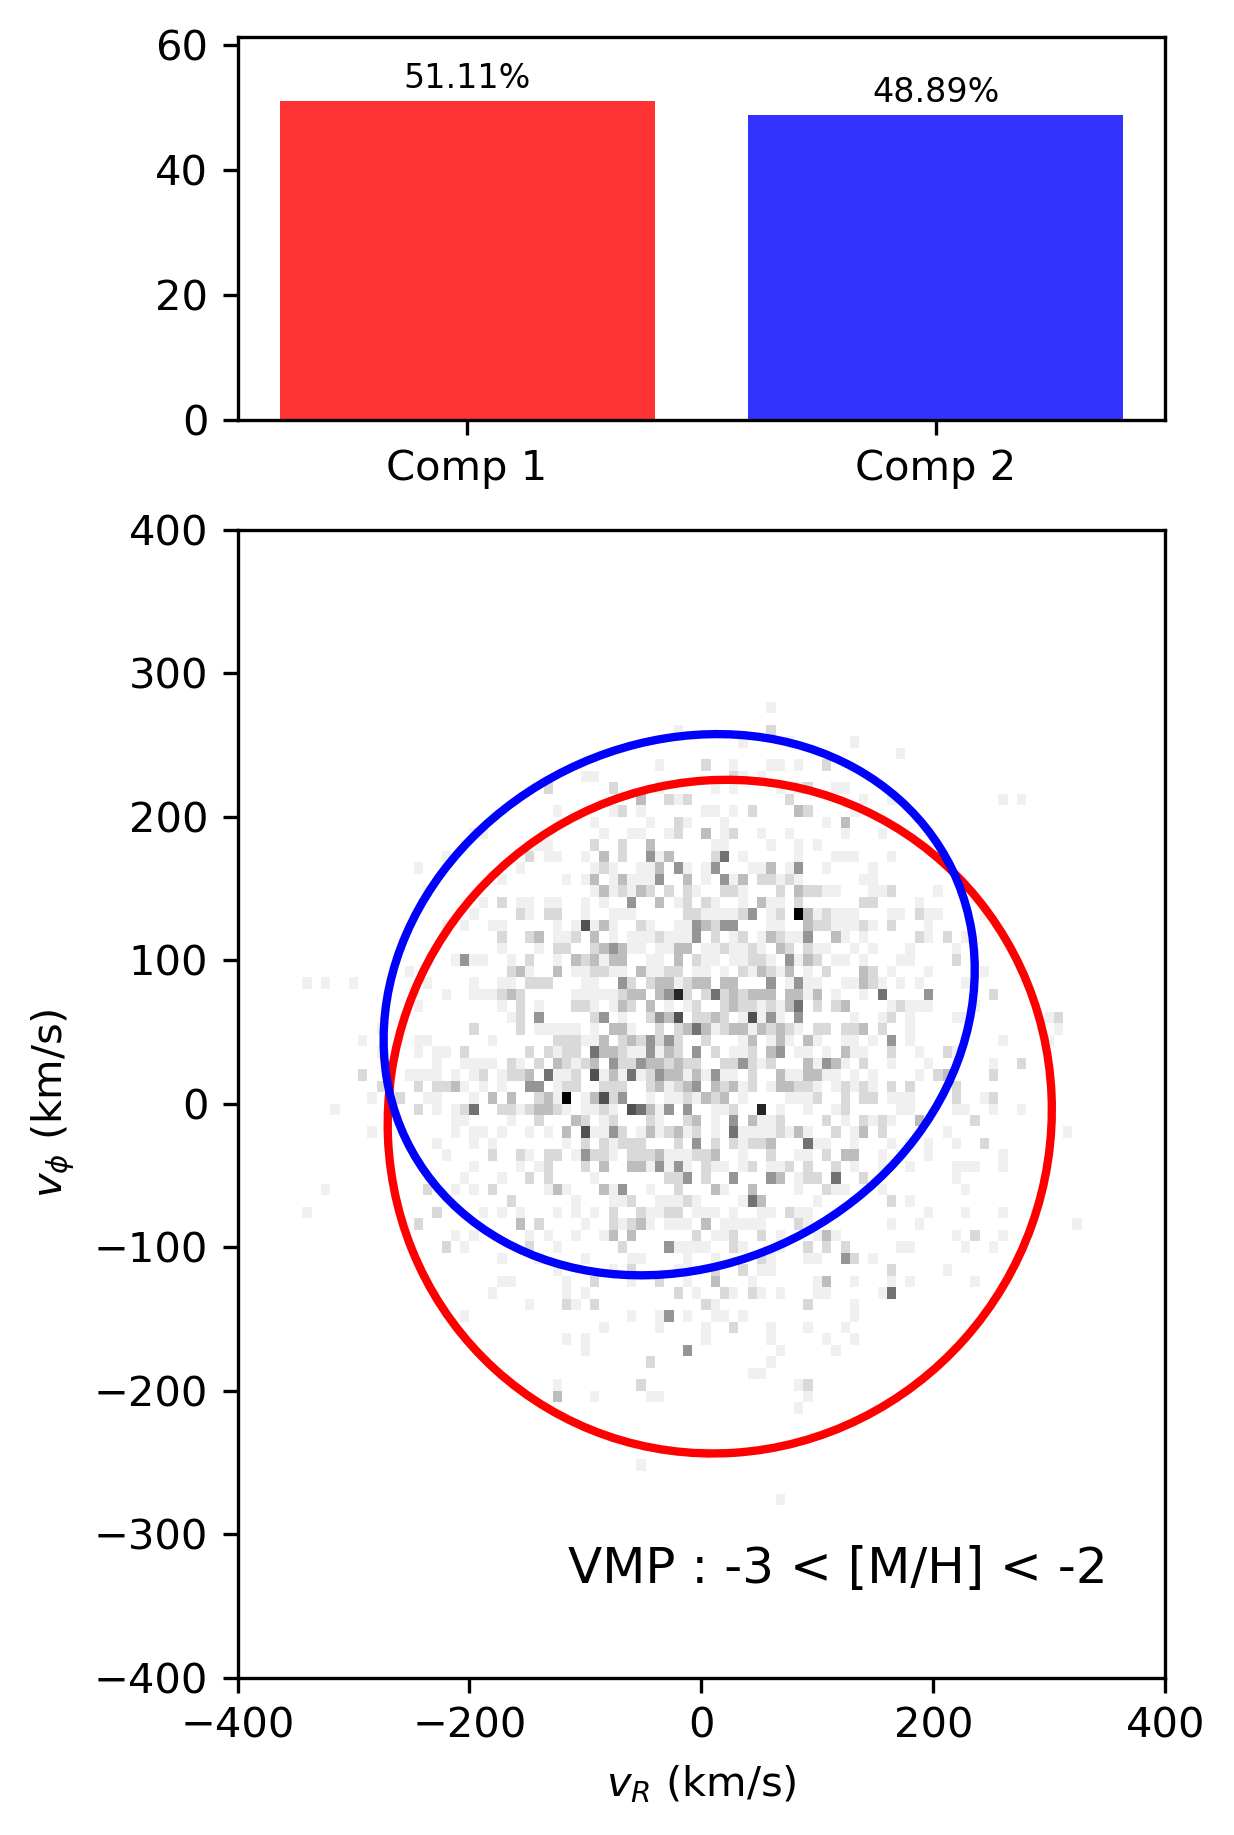
\includegraphics[width=\linewidth]{../figures/gmm_VMP.png}
  \end{subfigure}\hfill
  \begin{subfigure}[t]{0.245\textwidth}
    \centering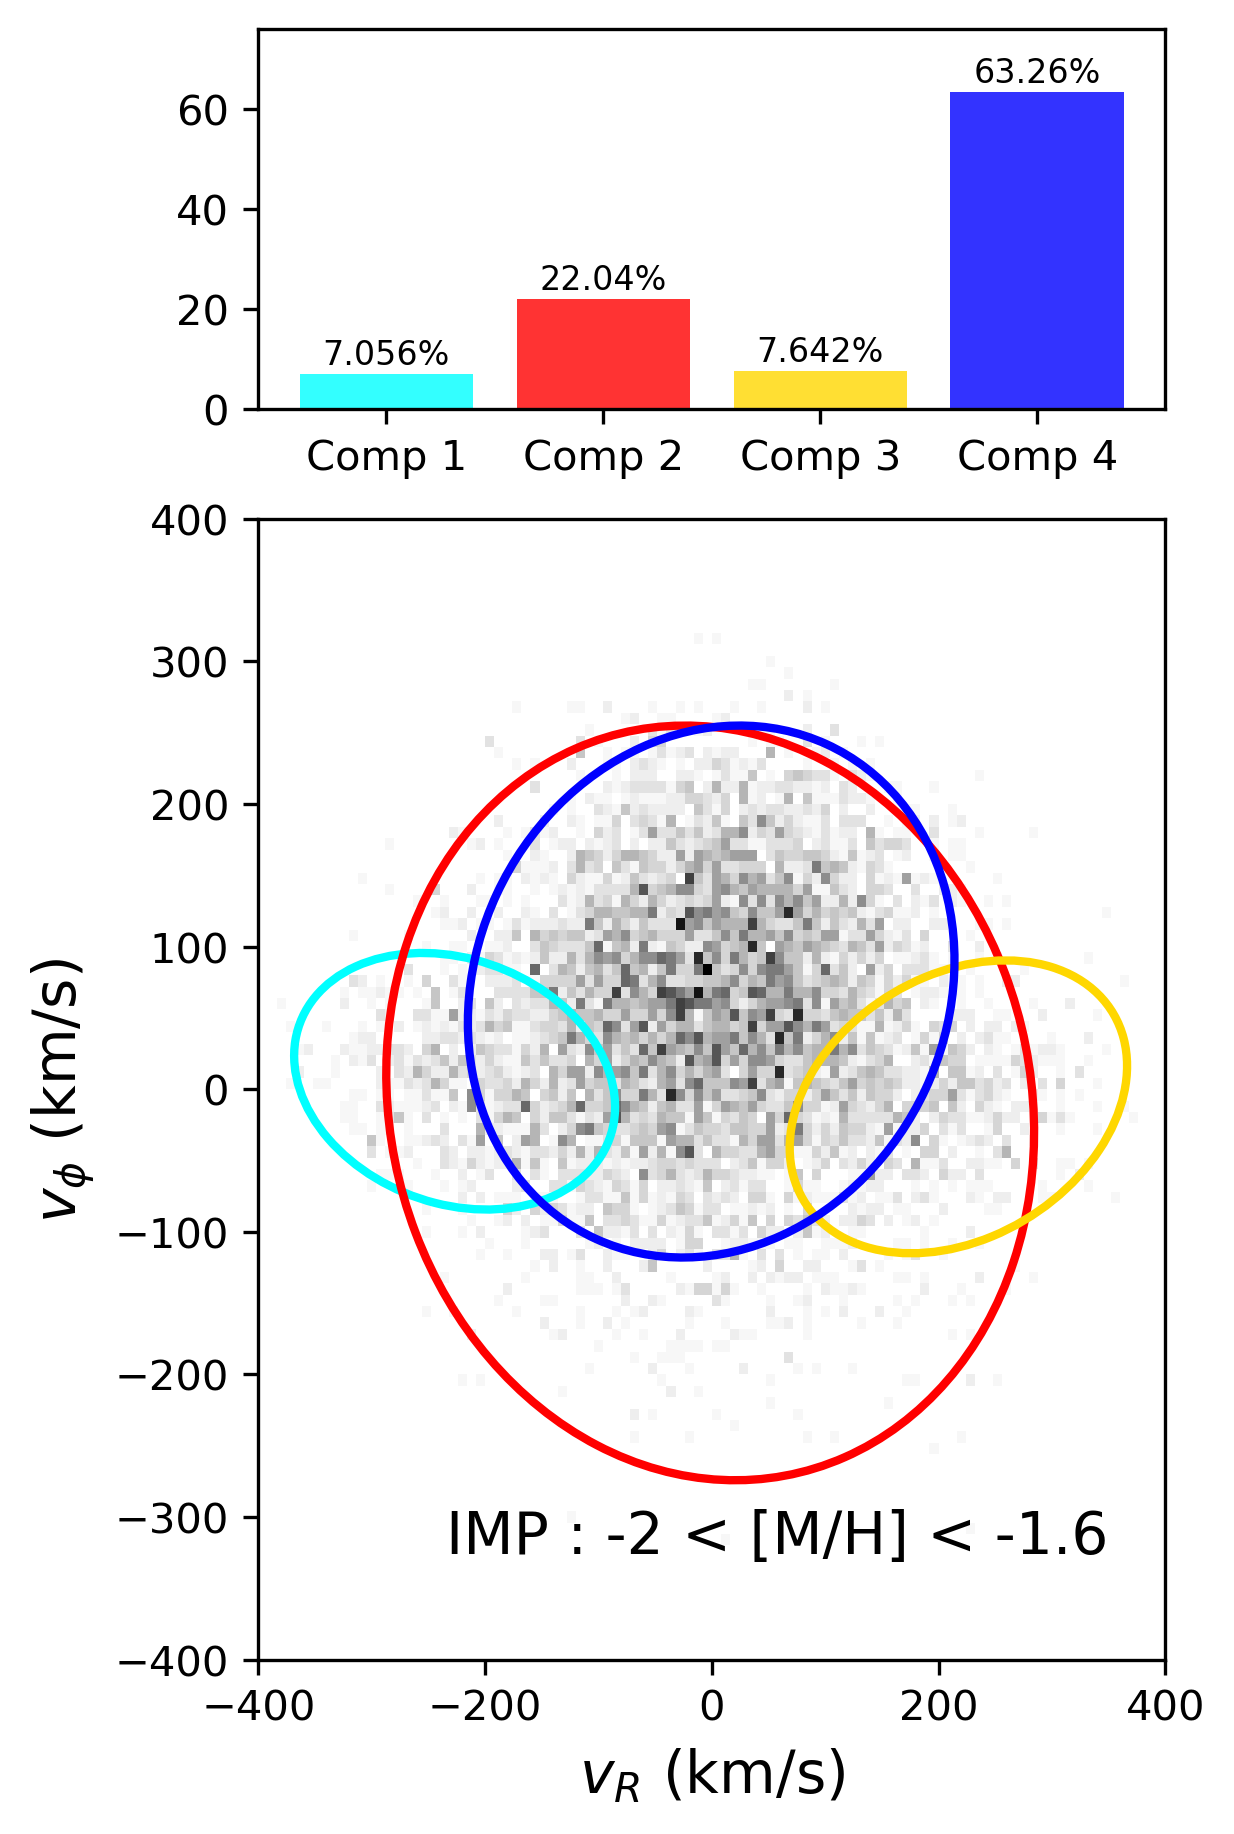
\includegraphics[width=\linewidth]{../figures/gmm_IMP.png}
  \end{subfigure}\hfill
  \begin{subfigure}[t]{0.245\textwidth}
    \centering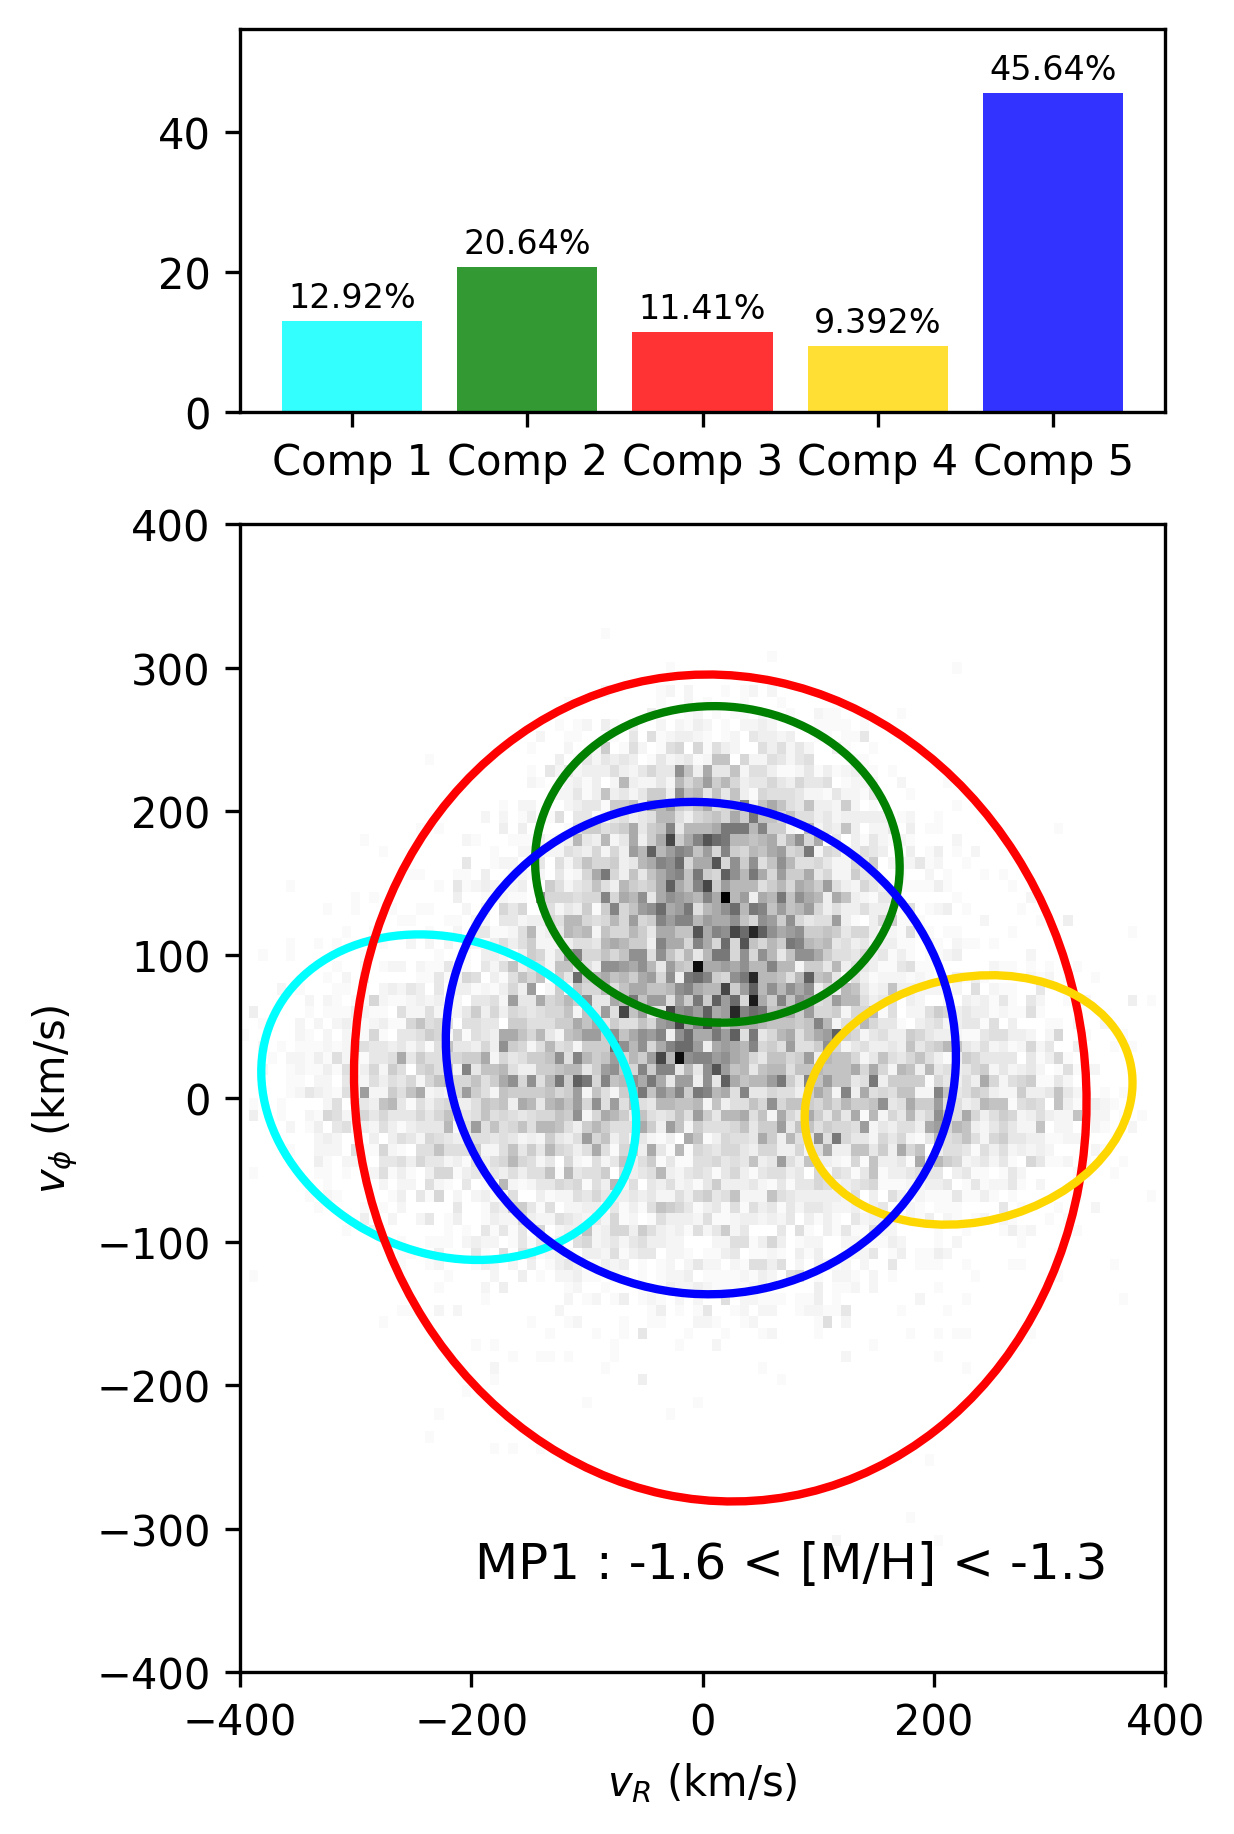
\includegraphics[width=\linewidth]{../figures/gmm_MP1.png}
  \end{subfigure}\hfill
  \begin{subfigure}[t]{0.245\textwidth}
    \centering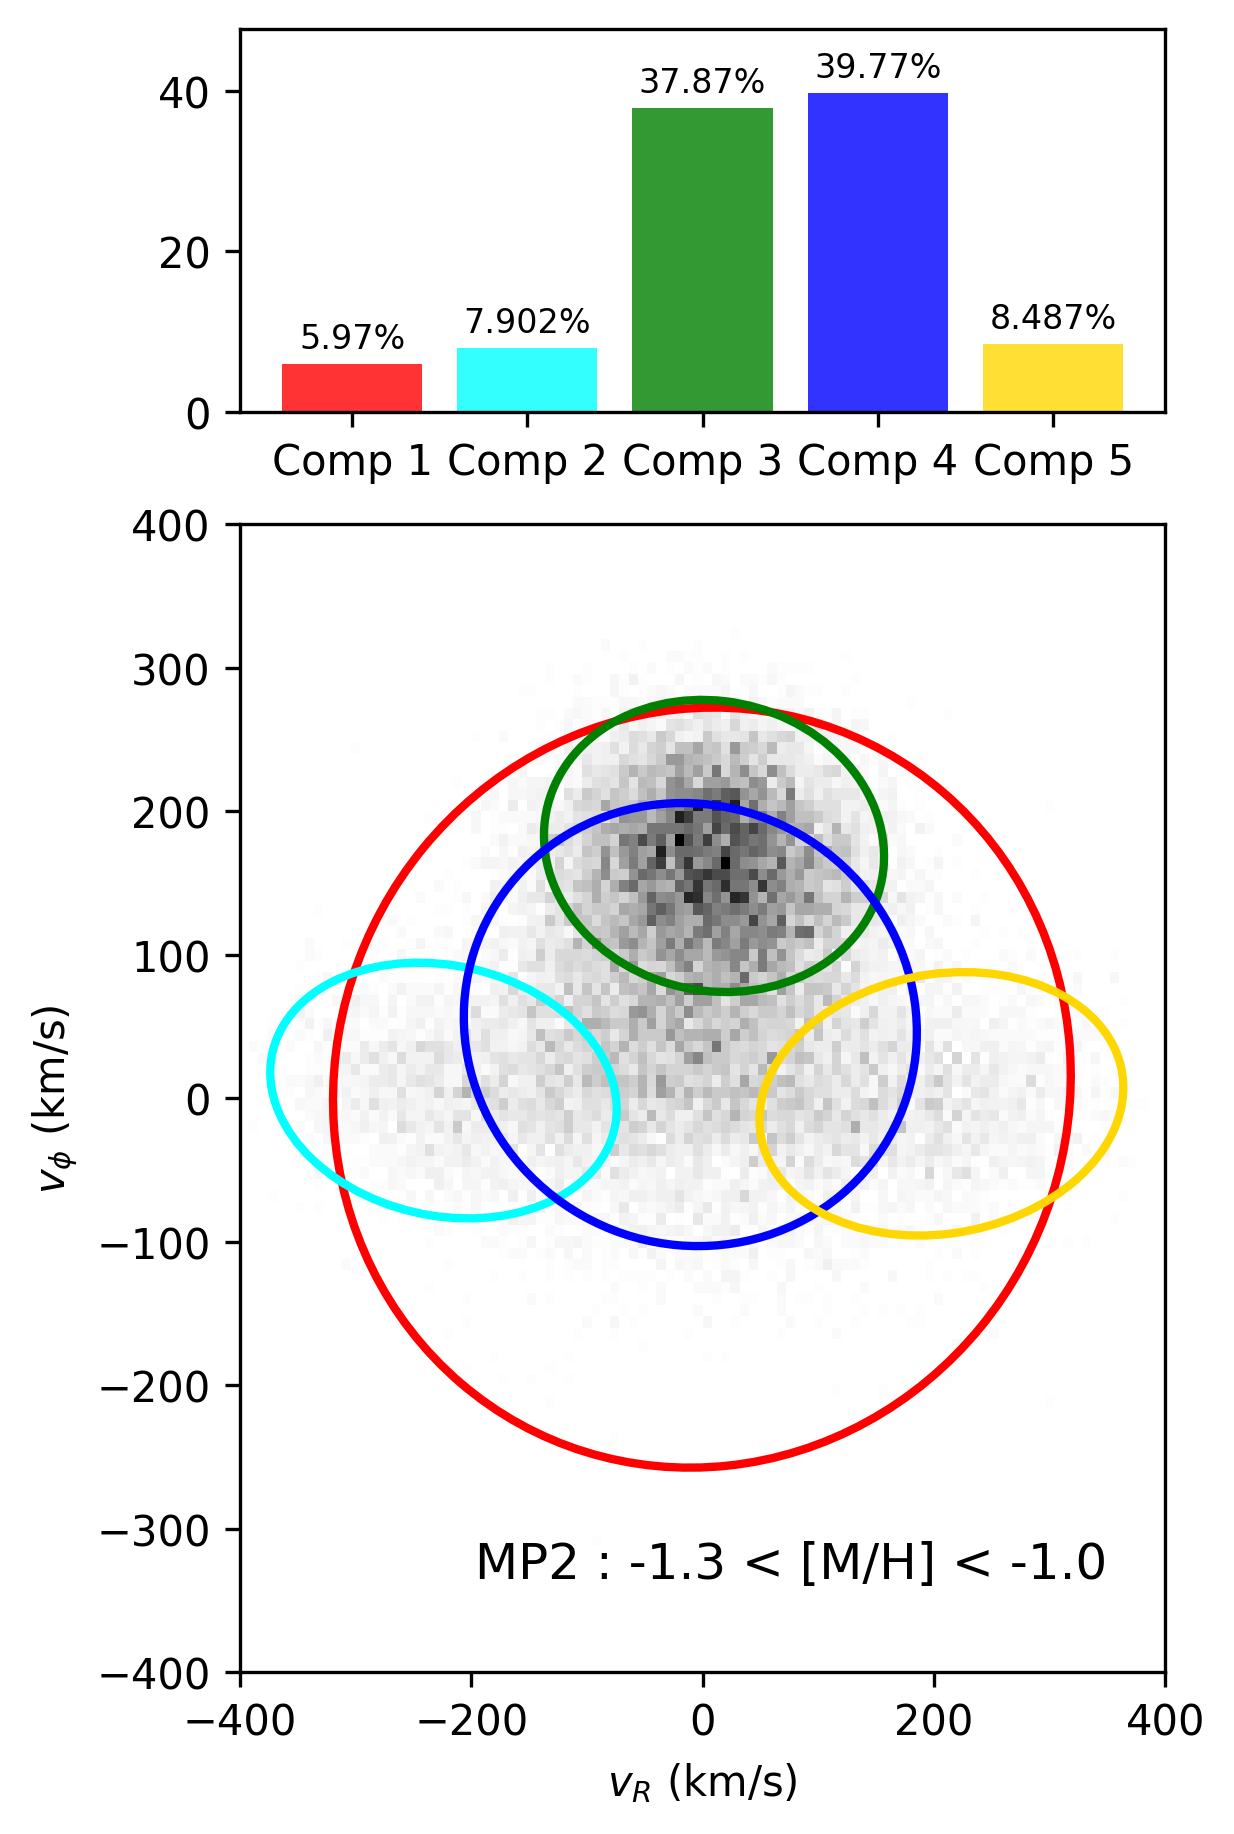
\includegraphics[width=\linewidth]{../figures/gmm_MP2.png}
  \end{subfigure}
  %
  \caption{\textbf{XD–GMM decomposition of metal-poor red-giant kinematics.}
           Each ellipse marks the $1\sigma$ contour of a Gaussian component in
           the $v_R$–$v_\phi$ plane.  From left to right the panels step up in
           metallicity, recovering the stationary–halo, prograde–halo and
           Gaia–Sausage/Enceladus structures reported by
           \citet{zhang2024existencemetalpoordiscmilky}, and revealing the
           first appearance of a thick-disc component above
           $\mathrm{[M/H]}\simeq-1.6$.}
  \label{fig:gmm_repro_zhang}
\end{figure*}


We extend the original method by splitting the sample into high- and low-$\alpha$ sequences \citep{Vis2024}, fitting separate 
XD-GMMs to each. By inspecting the component weights and kinematic properties, we quantify the emergence of rotational support 
and assess the presence of disc-like populations across both chemical tracks.

\subsection*{Key Findings}

Below $\mathrm{[M/H]}\!\simeq\!-1.6$ the velocity field of bright RGB stars is entirely halo–like: two hot Gaussians—one stationary, the other mildly prograde with $\bar{v}_{\phi}\!\approx\!70\;\mathrm{km\,s^{-1}}$—suffice to reproduce the data, and residual tests cap any hidden, rotation–supported disc at $\lesssim3$\,per~cent.  A warm disc component first appears in the $-1.6<\mathrm{[M/H]}<-1.3$ bin, carrying about one-fifth of the weight and rotating at $v_{\phi}\!\sim\!160\;\mathrm{km\,s^{-1}}$; by $-1.3<\mathrm{[M/H]}<-1.0$ it dominates ($\sim40$\,per~cent) and achieves $v_{\phi}/\sigma_{\phi}\!\gtrsim\!3$, signalling the birth of the thick disc.  Throughout $-2.0<\mathrm{[M/H]}<-1.0$ we also recover two highly radial Gaia–Sausage/Enceladus substructures that together account for $\sim$7–13\,per~cent of the sample and contribute no net rotation.

Splitting the data chemically sharpens the picture.  High-$\alpha$ stars acquire ordered rotation earlier: the thick-disc weight climbs from zero at $\mathrm{[M/H]}<-2$ to roughly one half by $\mathrm{[M/H]}\simeq-1.1$.  Low-$\alpha$ stars, in contrast, remain halo dominated until $\mathrm{[M/H]}>-1.3$ and only then develop a colder, thin-disc precursor (about one quarter of the population).  An unexpected GS/E signature appears within the high-$\alpha$ branch; its chemistry and kinematics suggest it stems from mis-classified, low-signal-to-noise abundances rather than an $\alpha$-rich progenitor.

Taken together, these results imply that coherent rotation became important once the interstellar medium reached roughly one-tenth solar metallicity, and that the rapid-formation (high-$\alpha$) population settled into a disc significantly earlier than the slower-forming (low-$\alpha$) branch—consistent with an inside-out, two-phase growth of the Milky Way.




\bibliographystyle{unsrt}  % Or use apalike, mnras, etc., depending on your needs
\bibliography{references}

% End of two-column content
\end{multicols}



\end{document}
